\subsection{Background}

\begin{landscape}
\begin{figure}
    \centering
    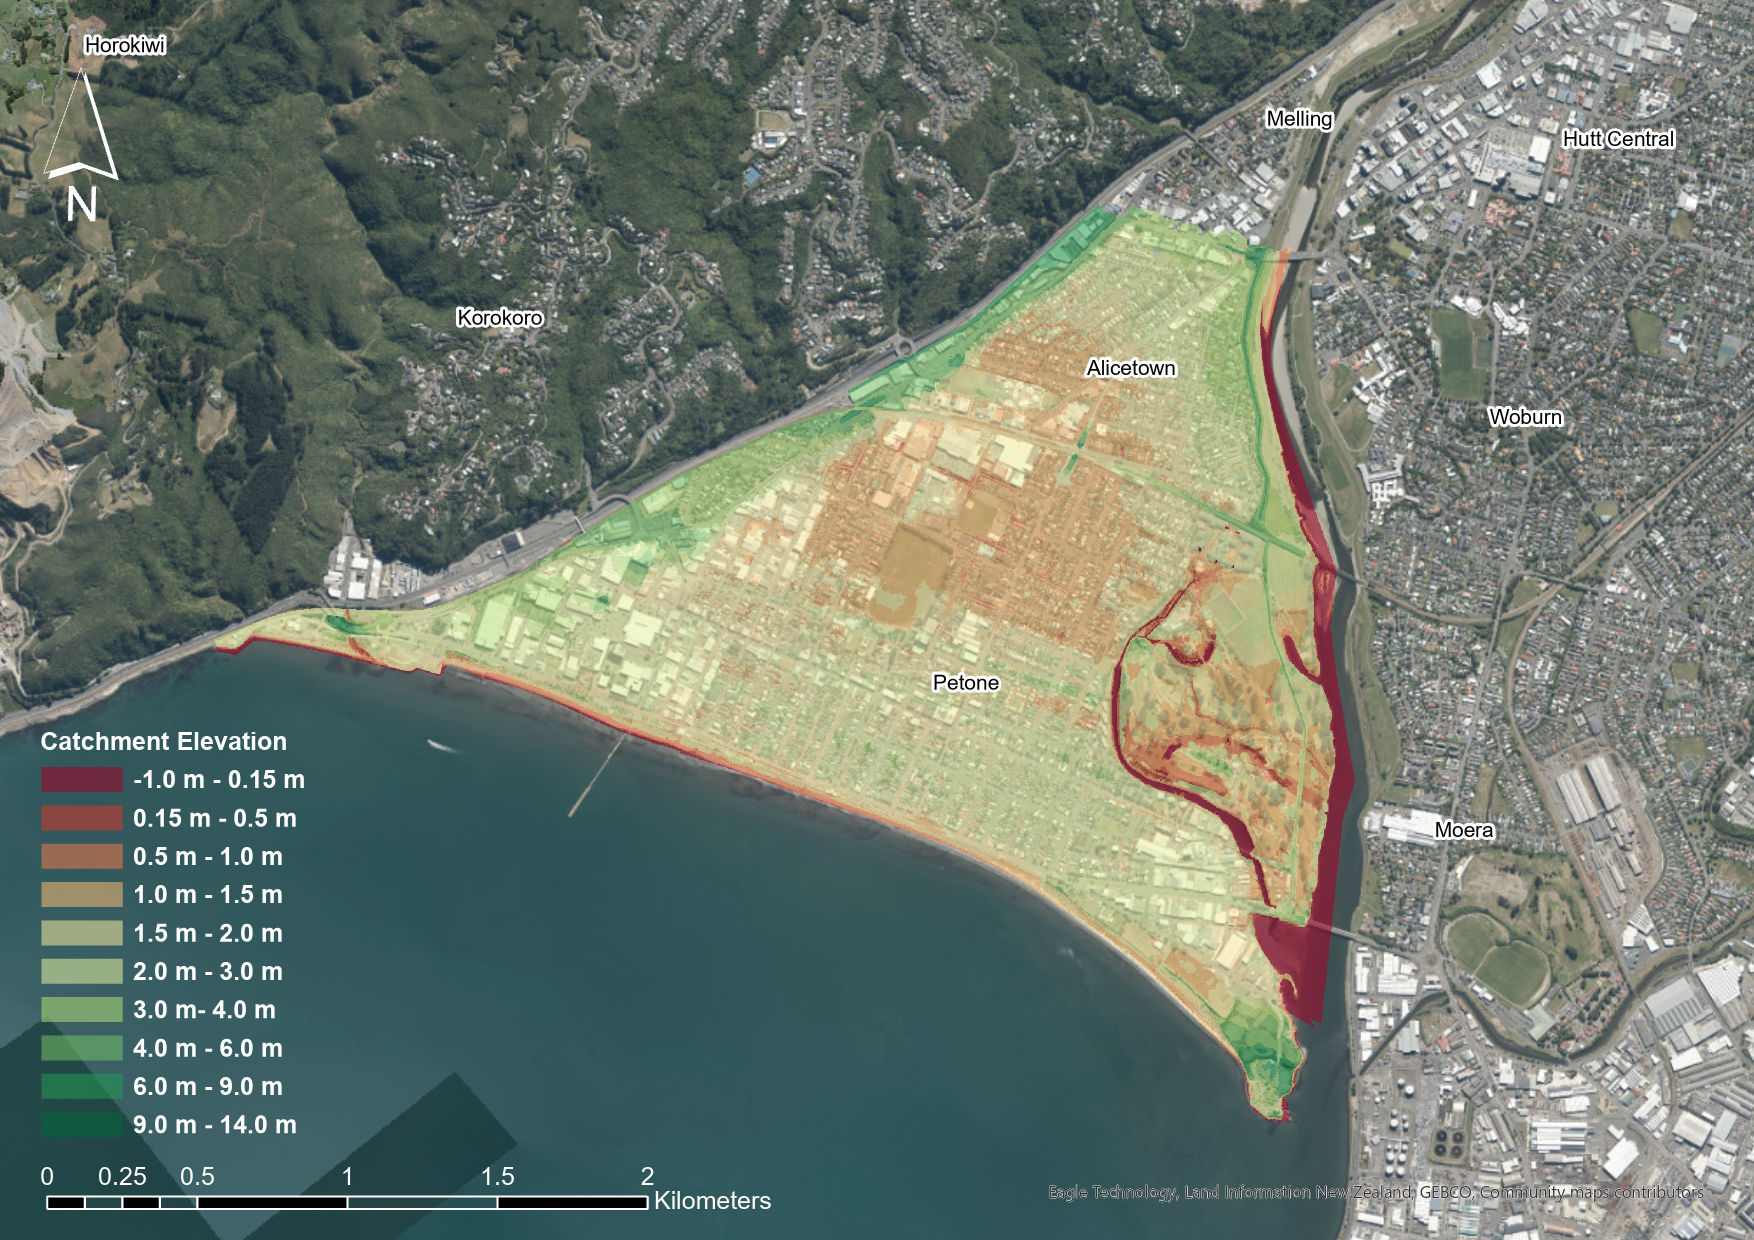
\includegraphics[width=1.0\linewidth]{Content/Figures/01_Introduction/Elevation-map.pdf}
    \caption{Elevation of Petone}
    \label{fig:elevation-map}
\end{figure}
\end{landscape}

\subsubsection{Case Study Area}

\begin{figure}
    \centering
    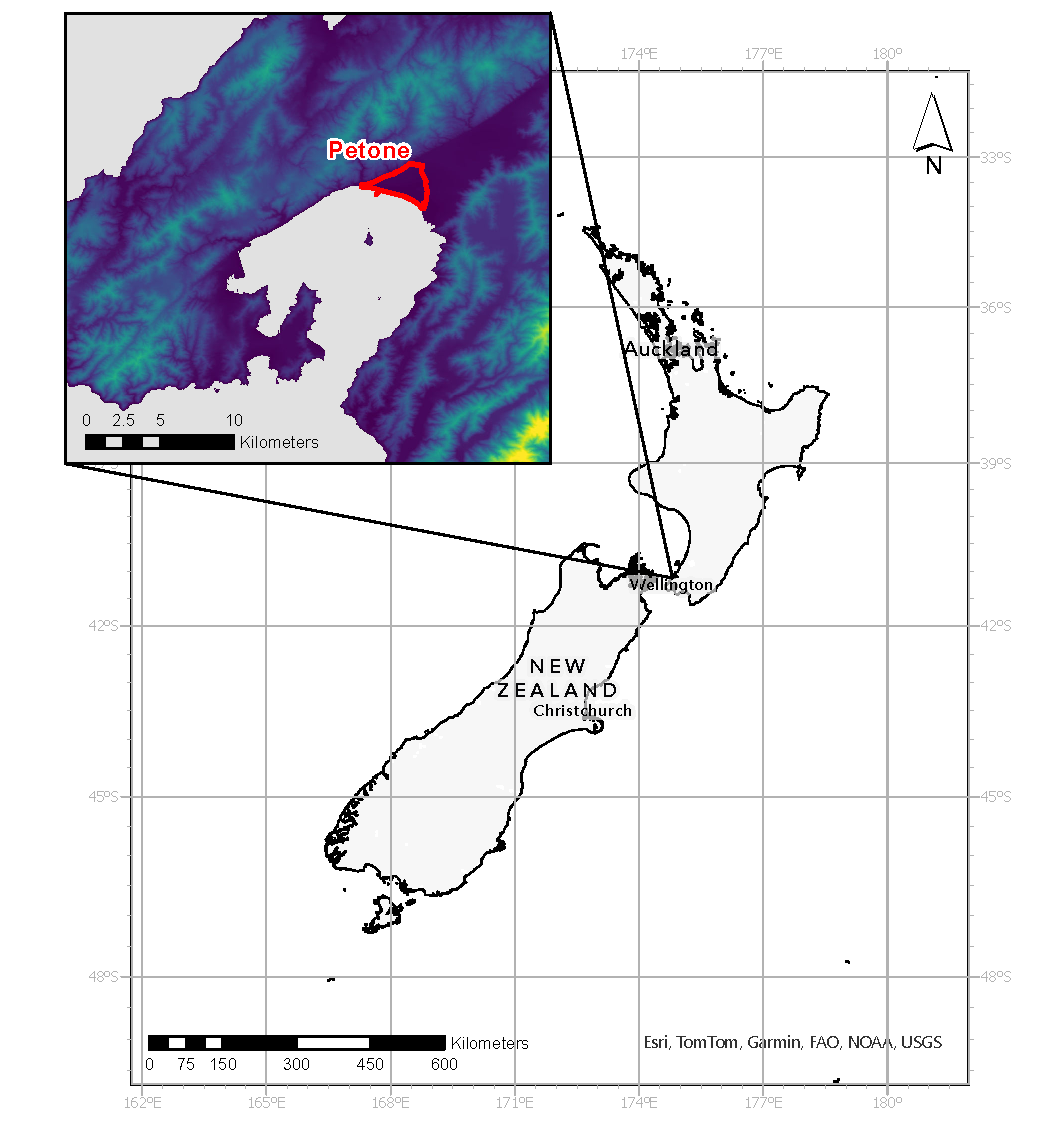
\includegraphics[width=1.0\linewidth]{Content/Figures/01_Introduction/study-area.pdf}
    \caption{Caption}
    \label{fig:enter-label}
\end{figure}

\subsection{Research Question}
\subsubsection{Research Objectives}
\begin{itemize}
    \item To identify which critical transport assets within the Petone-Alicetown catchment are vulnerable to flooding (coastal inundation, pluvial, fluvial) under current and future sea-level rise and climate scenarios as identified in the IPCC sixth assessment report and downscaled by NIWA (Andrews, 2023).
    \item To design and evaluate the technical feasibility of selected adaptation scenarios which highlight the use of NbS for addressing both coastal inundation and flooding from extreme rainfall compared to traditional grey infrastructure approaches, and to consider their role in a longer-term retreat strategy for Petone.
    \item To examine the cost-effectiveness of the selected adaptation options given the regulatory, financial, and governance barriers to their implementation within Hutt City’s existing urban transport system.
    \item To consider how the implementation of larger proposed transport projects (Cross Valley Link, River Link, Petone to Grenada) may: 
\begin{itemize}
    \item Alter the adaptation needs for the Petone-Alicetown catchment, and
    \item Be integrated with NbS adaptation options.
\end{itemize}
\end{itemize}




\subsection{Thesis Outline}

